\documentclass[12pt,a4paper]{article}
\usepackage{ryan}

\title{NUS Physics Engagement 2023}
\author{Ryan Joo}
\date{Last updated: \today}
\renewcommand{\arraystretch}{1.2}

\begin{document}

\maketitle
\tableofcontents
\pagebreak

\section{About the Programme}
\subsection{Schedule}
Day 1: 14 November 2023
\begin{table}[H]
\centering
\begin{tabular}{c|l}
\hline\hline
Time & Description \\
\hline
0930 -- 1030 & Opening address and talk by HOD \\
1040 -- 1140 & Lecture 1: Quantum materials by design for future devices \\
1140 -- 1245 & Lunch \\
1245 -- 1545 & Lab tours \\
1600 -- 1700 & Lecture 2: Black Holes: History of an idea \\
1700 -- 1800 & Dinner with Physics Seniors \\
\hline\hline
\end{tabular}
\caption{Schedule for Day 1}
\end{table}

Day 2: 15 November 2023
\begin{table}[H]
\centering
\begin{tabular}{c|l}
\hline\hline
Time & Description \\
\hline
0930 -- 1030 & Lecture 3: The physics of quantum communication \\
1040 -- 1140 & Lecture 4: Gravity: a relativist's guide to a broken theory \\
1140 -- 1240 & Lunch \\
1240 -- 1420 & Poster sharing session \\
1430 -- 1500 & Career prospects talk \\
1500 -- 1615 & Alumni panel session \\
1615 -- 1645 & Lucky draw \\
\hline\hline
\end{tabular}
\caption{Schedule for Day 2}
\end{table}

NUS Physics Department Telegram Channel: \url{t.me/NUSPHYS}
\pagebreak

\section{Lectures}
\subsection{Quantum Materials by Design for Future Devices}
{\color{red}\textit{Lecturer:}} \href{https://www.physics.nus.edu.sg/faculty/ariando/}{Prof. Ariando}

\subsubsection{Transistor}
\begin{figure}[H]
    \centering
    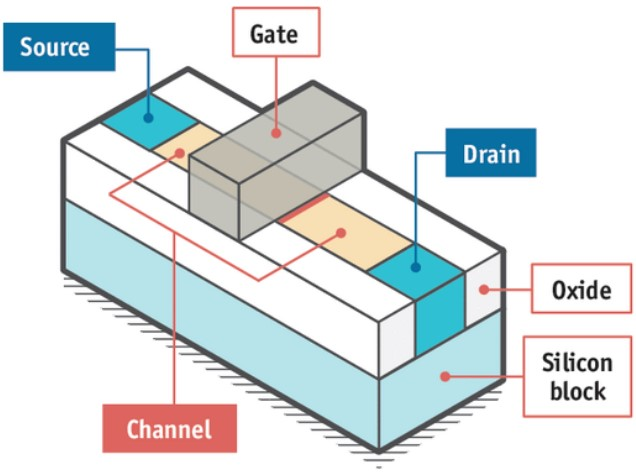
\includegraphics[width=8cm]{images/transistor.jpg}
    \caption{Transistor}
    \label{fig:transistor}
\end{figure}

Referring to \cref{fig:transistor}, a \textbf{transistor} is a sort of switch. To turn it on, a voltage is applied to its gate, which allows the current to flow through the channel between the transistor's source and drain. When no current flows, the transistor is off. The on-off states represent the 1s and 0s that are the fundamental language of computers.

In electronics, transistors are primarily made from semiconductor materials such as silicon (Si), and operate on the nanometre scale.

\subsubsection{Computing efficiency problem}
The \textbf{computing efficiency problem} arises in modern CPUs due to the substantial heat generated during operation. The central issue emerges from the increased power density resulting from the high number of transistors per unit area, as stipulated by Moore's Law. As these transistors become densely packed, the power utilisation can reach an overwhelming level, approximately 3 gigawatts (GW). This extensive power usage contributes significantly to the increasing heat generated within the CPU.

The primary source of this heat generation includes two significant factors:

\begin{itemize}
\item Charging of gate capacitor

Within the transistor, the process of charging and discharging the gate capacitor, a critical part of the transistor's function, consumes a notable amount of energy. This continuous charging and discharging cycle contributes to the overall thermal output.

\item Resistance of electron flow

As electrons move through the transistor, they collide with atoms, leading to atomic vibrations. Consequently, the kinetic energy of these collisions is transformed into thermal energy, adding to the heat dissipation.
\end{itemize}

The outcome of this excessive heat poses a challenge as it not only affects the CPU's performance but also escalates the risk of damage due to high temperatures. Efficient heat dissipation methods and novel technologies are continually being explored to address these challenges and maintain the trajectory outlined by \textbf{Moore's Law}\footnote{Moore's law is the observation and projection made by Gorden Moore -- co-founder of Fairchild Semiconductor and Intel -- that the number of transistors in an integrated circuit (IC) doubles about every two years.} in semiconductor innovation.

\subsubsection{Quantum material}
The use of quantum materials presents a promising approach to address the computing efficiency problem. In condensed matter physics, particularly in \textbf{strongly correlated electronic systems}, electron flow involves interactions among electrons that enable their navigation within a material, minimising collisions with atoms.

\textbf{Superconductivity} is a phenomenon exhibited by materials which possess the following two properties:
\begin{enumerate}
\item Conductor with zero resistance

Superconductivity is usually exhibited by superconductors at temperatures below a \textbf{critical temperature}, denoted by $T_C$. 

\begin{figure}[H]
    \centering
    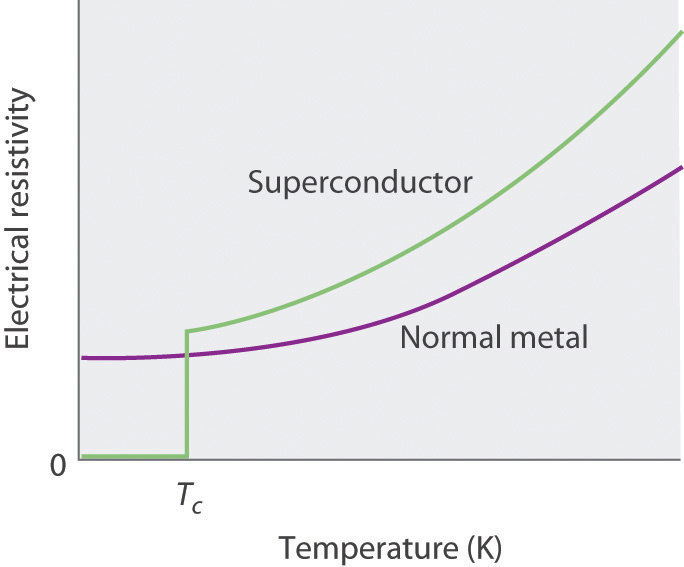
\includegraphics[width=8cm]{images/superconductivity_temp.jpg}
    \caption{Temperature-resistance graph}
    \label{fig:temp-resis_graph}
\end{figure}

In 1911, while studying the properties of matter at very low temperature, Dutch physicist Heike Kamerlingh Onnes discovered that the electrical resistance of mercury goes to zero below $4.2$ K (or $-269$\degree C) by cooling the metal using liquid helium. This was the very first observation of the phenomenon of superconductivity. Currently scientists are using machine learning to predict compounds that exhibit superconductivity, in particular at room temperature.

One theory to explain superconductivity is the \textbf{Bardeen--Cooper--Schrieffer (BCS) theory}. In this theory, electrons team up in what are called ``\textbf{Cooper pairs}". Normally, electrons repel each other due to their negative charges, making it harder for them to move without bumping into something, which creates resistance. But in superconductors, these electrons pair up and move together in a coordinated way, kind of like a dance where they avoid obstacles, as seen in \cref{fig:bcs_theory}. This teamwork reduces their chances of colliding with the atoms in the material, allowing them to move freely without losing any energy as heat. Hence these materials can conduct electricity without resistance when they are superconducting.

\begin{figure}[H]
    \centering
    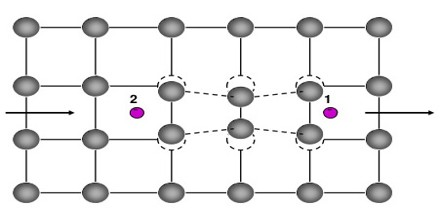
\includegraphics[width=8cm]{images/bcs_theory.jpg}
    \caption{Movement of electrons in superconductors}
    \label{fig:bcs_theory}
\end{figure}

\item Perfect expulsion of magnetic field

A notable effect linked to superconductivity is the \textbf{Meissner effect}, the observation where materials exhibit magnetic repulsion, leading to magnetic levitation, as is seen on Maglev trains that can travel at very high speeds.

\begin{figure}[H]
    \centering
    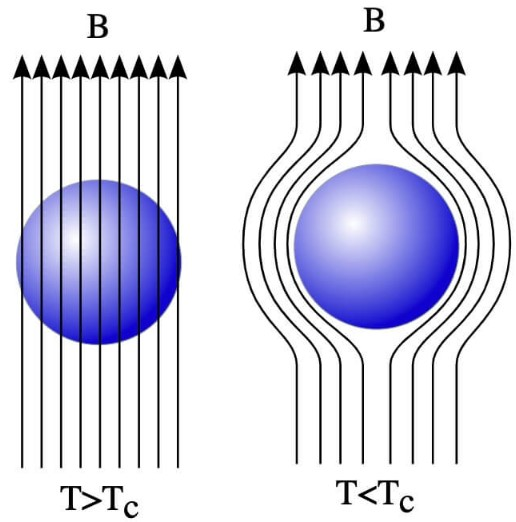
\includegraphics[width=6cm]{images/superconductivity_mag.jpg}
    \caption{Magnetic field of superconductors}
    \label{fig:maglev}
\end{figure}
\end{enumerate}
\pagebreak

\subsection{Black Holes: History of An Idea}
{\color{red}\textit{Lecturer:}} \href{https://www.physics.nus.edu.sg/faculty/teo-ho-khoon-edward/}{A/Prof. Edward Teo}

\subsubsection{Escape velocity and Schwarzschild radius}
The \textbf{escape velocity} of a celestial body is the minimum velocity required to escape from its gravitational effect. From A Level Physics, the formula for the escape velocity $v$ of an object of a distance $r$ from the centre of a planet of mass $M$ (assuming all the mass is concentrated at a single point) can be easily deduced:
\begin{equation}\label{escape_velocity}
v = \sqrt{\frac{2GM}{r}}
\end{equation}

For a star of constant density, it is evident that when $r$ is doubled, $M$ is multiplied 8 times, so $v$ is doubled. Hence one might deduce that for a star about 500 times the mass of our Sun, the escape velocity will be equal to the speed of light, which means that the star should be a black hole as we know it, since even light cannot escape its gravitational effect. However, in reality, this is not true as for larger stars (which are usually made up of gas), the gas spreads out to a larger extent, which lowers the density of the star.

Moving on, suppose we compress a celestial body to become a black hole such that light cannot escape its gravitational effect, then the maximum radius of the compressed body is known as the \textbf{Schwarzschild radius}, the formula of which can be easily deduced from \cref{escape_velocity} by substituting $v=c$:
\begin{equation}
r_s = \frac{2GM}{c^2}
\end{equation}

\subsubsection{Our Sun}
The first \textbf{spectograph} of the Sun, as seen in \cref{fig:spectograph}, contains absorption lines in its spectrum, indicating the composition of elements present on its surface, such as hydrogen (H) and helium (He), among others.

\begin{figure}[H]
    \centering
    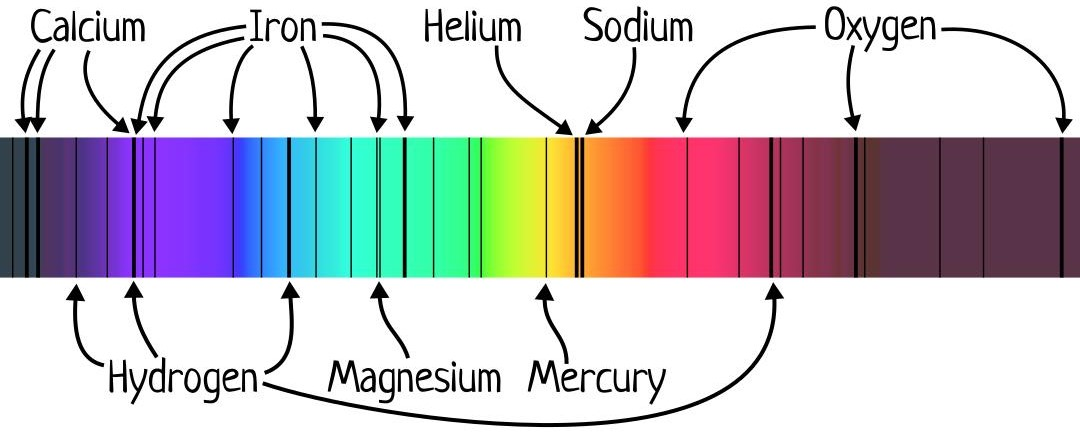
\includegraphics[width=10cm]{images/spectograph_sun.jpg}
    \caption{Spectograph of our Sun}
    \label{fig:spectograph}
\end{figure}

The Sun primarily generates energy through \textbf{nuclear fusion}, specifically through a process called the \textbf{proton--proton chain reaction}. In this sequence of reactions, hydrogen nuclei (protons) fuse together, forming helium nuclei and releasing energy in the form of light and heat.

\begin{align*}
&\ce{^1H + ^1H -> ^2H + e^+ + \nu} \\
&\ce{^2H + ^1H -> ^3He + \gamma} \\
&\ce{^3He + ^4He -> ^7Be + \gamma} \\
&\ce{^7Be + e^- -> ^7Li + \nu} \\
&\ce{^7Li + ^1H -> ^4He + ^4He}
\end{align*}

Note that the overall reaction is \ce{4 ^1H -> 1 He}.

The above nuclear fusion reactions generates an outward thermal pressure. When the gravitational force balances the thermal pressure, a stable equilibrium is achieved. This balance maintains the star's size, known as its radius, keeping it relatively constant over a prolonged period, which explains the observed stability of the Sun's radius.

When the hydrogen fuel in a star's core is exhausted, the above sequence of reactions comes to a stop. Thermal pressure is no longer emitted out to balance gravitational force, so the net inwards force compresses the star, increasing the pressure and temperature. This compression initiates the fusion of helium into heavier elements such as carbon. This fusion process continues, leading to the creation of even heavier elements in larger stars, eventually culminating in the fusion of elements to form iron (Fe), which marks the most stable state in terms of nuclear reactions within stars.

\subsubsection{Electrons}
Electrons were discovered by Thomson. Then Pauli came up with the \textbf{Pauli exclusion principle}, which states that electrons cannot occupy the same space as electrons belong to \textbf{fermions}, a group of particles; this means that there is a point where gas can no longer be compressed.

When a star is continued to be compressed, electrons are compressed side-by-side to form a \textbf{white dwarf}. Electron degeneracy pressure generates an outward force to balance the inward gravitational force, which halts the gravitational collapse of a star. There is a limit to this: the maximum mass of a star that compressed only until a white dwarf and does not continue collapsing is known as the \textbf{Chandrasekhar limit} (1.44 solar masses).

If the mass of the star is greater than the Chandrasekhar limit, then it will be compressed to a \textbf{neutron star}, which completely consists of neutrons, as electrons combine with protons to form neutrons.

\subsubsection{Neutrons}
Similarly, as gravitational force is greater than the neutron degeneracy pressure, a neutron star with a mass greater than 3 solar masses will collapse to form a \textbf{black hole}.

Since neutrons are also a type of fermions and are not electrically charged, they can pack more closely together than electrons, making a neutron star much more dense than a white dwarf.

\subsubsection{Black holes}

Einstein's theory of relativity comprises two fundamental concepts: special relativity and general relativity. \textbf{Special relativity} postulates that the speed of light $c$ is constant for all observers, time is considered a fourth dimension, and introduces the famous equation $E=mc^2$ relating energy and mass. On the other hand, \textbf{general relativity} describes gravity as the curvature of spacetime caused by mass and energy.

The \textbf{Schwarzschild solution} describes the gravitational field in a vacuum outside a spherically symmetric, non-rotating mass, often used as a model for a black hole.

\begin{equation}
\dd{s^2} = -\brac{1-\frac{r_s}{r}}\dd{t^2} + \frac{\dd{r^2}}{1-\frac{r_s}{r}} + r^2(\dd{\theta^2}+\sin^2\theta\dd{\phi^2})
\end{equation}

Gravitational collapse solution

Gravitational time dilation can be derived from Schwarzschild solution, which is given by
\begin{equation}\label{g-time-dilation}
\frac{\Delta T}{\Delta t} = \sqrt{\frac{1-\frac{r_s}{r}}{1-\frac{r_s}{R}}} > 1
\end{equation}
This suggests that gravity slows time down. For smaller $R$, since speed of light is constant and $E \propto f$, light loses energy so frequency $f$ decreases while wavelength $\lambda$ increases, resulting in redshifting of colour of light.

As $R \to r_s$, the denominator of \cref{g-time-dilation} tends to zero so $\Delta T \to \infty$ which indicates an infinite slow down of time. Taking limits, time comes to a stop/standstill and redshift becomes infinite (which means that light can no longer be observed, which explains its disappearance from view).

The \textbf{event horizon} is when $R=r_s$.

The \textbf{Oppenheimer--Snyder solution} describes the collapse of a star (assuming pressureless for $r\le R$), as seen in \cref{fig:oppenheimer_snyder}. All matter falls towards $r=0$ -- \textbf{singularity}, the point of zero size and thus infinite density -- in \emph{finite proper time}\footnote{time measured by matter itself}. Referring to \cref{fig:oppenheimer_snyder}, as time increases from $t=0$, gravity causes light to bend as light is attracted to the black hole; for $r \le r_s$, light no longer travels beyond the event horizon where $r=r_s$.

\begin{figure}[H]
    \centering
    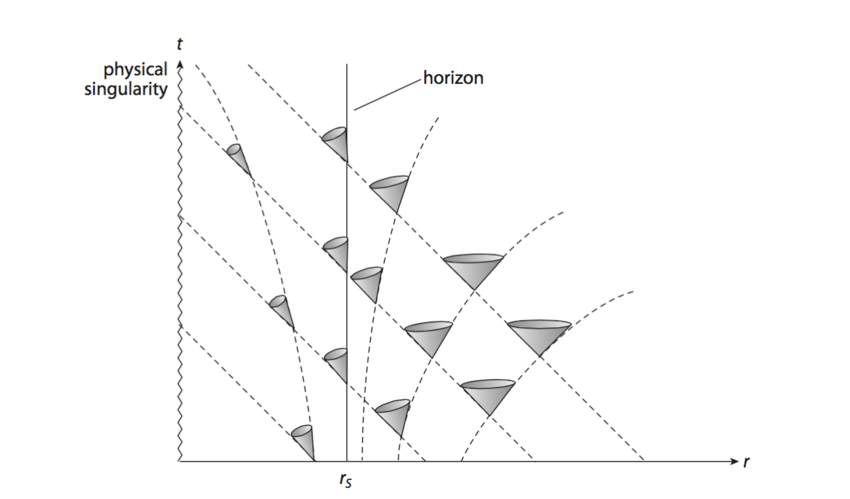
\includegraphics[width=17cm]{images/oppenheimer_snyder.png}
    \caption{Light cones in space-time plane}
    \label{fig:oppenheimer_snyder}
\end{figure}

Other further topics that you can read up on include: Kerr solution for a rotating black hole, Penrose diagram, no-hair theorem, Hawking radiation.
\pagebreak

\subsection{The Physics of Quantum Communication}
{\color{red}\textit{Lecturer:}} \href{https://www.physics.nus.edu.sg/faculty/ling-euk-jin-alexander/}{A/Prof. Alexander Ling}

\subsubsection{Quantum bit}
In classical computing, \textbf{bits} store information as either a 0 or a 1, with the state constantly shifting between these two values. Quantum computing introduces \textbf{qubits}, which operate using quantum phenomena such as the spin of electrons, superconductor properties, or photons to store information. Unlike classical bits, qubits can exist in a state of \textbf{superposition}, which means the simultaneous existence of both states of 0 and 1 until measured, offering a potentially exponential increase in computational power and capability. This ability to hold multiple states at once forms the basis of quantum computing's enhanced processing potential.

\begin{equation}\label{quantum_bit}
\ket{a} = \frac{1}{\sqrt{2}}\brac{\ket{0}+\ket{1}}
\end{equation}
where $\ket{0}$ and $\ket{1}$ denote the proportion of 0s and 1s.

Quantum technologies have broad applications across various fields:
\begin{itemize}
\item Secure communication: Quantum encryption leverages the principles of quantum mechanics to develop secure communication protocols. It utilizes quantum properties to encode information, making it theoretically impossible to intercept without detection.

\item Quantum computing: Quantum computers have the potential to revolutionize computing by performing complex calculations at an exponentially faster rate compared to classical computers. They utilize qubits, capitalizing on principles like superposition and entanglement for advanced data processing.

\item Metrology: Quantum-based sensing technologies enable highly precise measurements. Quantum metrology uses quantum systems to detect and measure physical quantities with exceptional accuracy, contributing to advancements in fields like navigation, timekeeping, and environmental monitoring.
\end{itemize}

\subsubsection{Light}
Light behaves according to classical physics, adhering to principles of optics. Some key concepts include:
\begin{itemize}
\item Speed, frequency, wavelength

Light travels at a constant speed $c$ in a vacuum and is characterised by its frequency $f$ and wavelength $\lambda$.

\begin{equation}
c=f\lambda
\end{equation}

\item Refractive index

When light travels through a medium with a refractive index $n$, its speed changes to $c = \frac{c_0}{n}$, and the wavelength also changes to $\lambda = \frac{\lambda_0}{n}$.

\begin{equation}
c=\frac{c_0}{n}, \quad \lambda=\frac{\lambda_0}{n}
\end{equation}

\item Polarisation of electromagnetic field

Light exhibits polarisation, where the electric field oscillates in a specific direction.

\item Quantum nature of light

Although light primarily follows classical physics, it also exhibits particle-like behavior, known as photons, when observed in quantum mechanics.
\end{itemize}

It is possible to build quantum systems using traditional optical elements and techniques such as optical fibres, often in applications such as quantum communication and computation.

The \textbf{Gaussian beam} equation describes the intensity $I$ of a beam at a distance $z$ from its source, influenced by parameters such as distance from the beam axis $r$ and beam width $w(z)$.

\begin{equation}
I(r,z) = I_0\brac{\frac{w_0}{w(z)}}^2\exp\brac{\frac{-2r^2}{w(z)^2}}
\end{equation}
where $w_0$ denotes the smallest beam width.

\textbf{Polarisation degree of freedom} of a photon refers to the various orientations or states that the electric field component of an electromagnetic wave can adopt. This property describes the direction in which the electric field oscillates as the wave propagates. One of the types of polarisation is linear polarisation, where light can be either \textit{horizontally} or \textit{vertically} polarised.

\begin{equation}\label{polarisation_photon}
\ket{a} = \frac{1}{\sqrt{2}}\brac{\ket{H}+\ket{V}}
\end{equation}
where $\ket{H}$ and $\ket{V}$ denote the probability of a photon being either horizontally or vertically polarised. Notice that \cref{polarisation_photon} is analogous to \cref{quantum_bit}.


The \textbf{Uncertainty Principle} -- formulated by Heisenberg -- posits that it is impossible to precisely measure both the position and momentum of a particle simultaneously. This principle suggests an inherent limit to the precision with which certain pairs of properties, such as position and momentum, can be known; the more accurately one property is measured, the less accurately the other can be determined.

The \textbf{No-cloning Theorem} -- proposed by physicists Wootters and Zurek -- states that an arbitrary unknown quantum state cannot be precisely copied or cloned. In other words, if the exact state of a quantum particle is unknown, it cannot be replicated perfectly. This theorem underscores the unique and non-reproducible nature of quantum information.

\subsubsection{Generation of entangled states}
Generating entangled states involving more than one qubit often involves specific quantum processes. One such method is through the phenomenon of \textbf{spontaneous parametric down-conversion (SPDC)}, which occurs in certain nonlinear crystals. When a high-energy photon, typically from a laser, interacts with a nonlinear crystal, it can split into two lower-energy photons. These photons emerge in pairs: the \textbf{signal} photon and the \textbf{idler} photon. Importantly, due to the conservation laws of energy and momentum, these photons are entangled. The properties of these entangled photons, such as their polarisation or spin states, become correlated. Measuring one of the entangled photons instantaneously determines the state of the other, no matter the distance separating them.

\begin{equation}
\ket{\Phi^+} = \frac{1}{\sqrt{2}}\brac{\ket{H}_1 \otimes \ket{H}_2 + \ket{V}_1 \otimes \ket{V}_2}
\end{equation}
where there are 2 qubits. The two qubits generated have a strong correlation between them; if qubit 1 is in horizontal polarisation, then by correlation qubit 2 must also be in horizontal polarisation.

\subsubsection{Quantum key distribution}
\textbf{Quantum key distribution (QKD)} systems employ entangled particle sources, such as entangled photon pairs, to generate cryptographic keys. Here is an overview of the process:

\begin{enumerate}
\item Entangled particle generation:

A source produces entangled particle pairs, such as photons, in an entangled state. For instance, a process such as SPDC can generate entangled photon pairs.

\item Transmission:

The entangled particles are separated and sent to two different locations: typically the sender (Alice) and the receiver (Bob).

\item Polarisation encoding:

Alice encodes information onto her photons using different polarisations. She chooses measurement bases (e.g. horizontal/vertical or diagonal) to encode the cryptographic information.

\item Measurement and correlation:

Bob receives the photons and measures their polarisations using chosen bases. As per quantum rules, his measurements are random. However, when Alice and Bob compare the bases used for encoding and measuring, they get correlated results due to entanglement.

\item Error rate estimation:

Some measured photons will not match due to measurement discrepancies or environmental interference. By comparing a subset of their measurements, Alice and Bob can estimate the error rate.

\item Key distillation:

They discard mismatched measurements and extract a subset of matching bits to form a secure quantum key, which they can use for encryption.

\item Security verification:

To ensure the security of the key, Alice and Bob perform additional checks, such as privacy amplification, to guarantee that the remaining key is secure against potential eavesdropping.
\end{enumerate}

The fascinating aspect is that any attempt to intercept or measure the entangled particles during transmission would break the correlation between photons. This disturbance would be detectable as errors in the key, alerting Alice and Bob to potential eavesdropping attempts.
\pagebreak

\subsection{Gravity: A Relativist's Guide to A Broken Theory}
{\color{red}\textit{Lecturer:}} \href{https://sg.linkedin.com/in/josh-mathews-190901116}{Dr. Josh Matthews}

\subsubsection{Gravity}
The progress in understanding gravity owes much to Galileo's observations, Kepler's laws of planetary motion, and Newton's formulation of universal gravitation.

However, as scientific exploration advanced, challenges emerged that questioned the adequacy of Newtonian physics. Observations of the orbit of Mercury highlighted a discrepancy: its elliptical orbit showed a gradual shift caused by gravitational influences from other celestial bodies, deviating slightly from the predictions of Newtonian gravity. Moreover, the constant speed of light, as expounded in Einstein's special theory of relativity, contradicted Newtonian physics. Newton's laws didn't adequately accommodate the fixed nature of the speed of light, especially in scenarios involving intense gravitational fields and high velocities.

\subsubsection{General relativity}
Einstein's theories of relativity transformed our understanding of space, time, and gravity. \textbf{Special relativity} introduced the famous mass--energy equivalence equation
\begin{equation}
E=mc^2
\end{equation}
demonstrating that energy and mass are interchangeable. It also established that the speed of light $c$ remains constant for all observers, regardless of their motion.

\textbf{General relativity} conceptualises gravity not as a force but as the consequence of the curvature of spacetime caused by mass and energy. The presence of mass and energy curves the fabric of spacetime, and objects move along curved paths due to this curvature, creating the effect we interpret as gravity.

The field equations of general relativity, often represented by
\begin{equation}
G_{\mu\nu} = \frac{8\pi G}{c^4}T_{\mu\nu}
\end{equation}
describes the relationship between the curvature of spacetime (expressed by $G_{\mu\nu}$) and the distribution of matter and energy (represented by $T_{\mu\nu}$).

The 1919 solar eclipse observed in West Africa was a pivotal event that provided experimental evidence supporting Einstein's general theory of relativity. During the eclipse, astronomers observed starlight passing near the Sun. The light from the stars was slightly bent by the Sun's gravitational field, causing a slight shift in their apparent positions in the sky. This observation confirmed the gravitational bending of light as predicted by Einstein's theory, validating the concept that massive objects like the Sun can bend the path of light.

\textbf{Pulsars} are rapidly rotating neutron stars that emit beams of radiation from their magnetic poles. These beams are observed as pulses of radiation when they sweep across the Earth, giving rise to the name ``pulsar". The regularity of these pulses is attributed to the pulsar's rotation, akin to a cosmic lighthouse. \textbf{Pulsar binaries} are systems in which a pulsar is in orbit with another celestial body, often a companion star.

Despite its profound explanatory power, general relativity encounters challenges in explaining certain astronomical phenomena:
\begin{itemize}
\item Dark matter refers to unseen matter inferred from gravitational effects
\item Dark energy relates to the observed accelerated expansion of the universe.
\item The singularity within a black hole, where the laws of physics break down, remains an enigmatic point. 
\item Reconciling general relativity with quantum mechanics, particularly at the extreme conditions within a black hole or during the early universe, remains a significant unresolved challenge in modern physics.
\end{itemize}

\subsubsection{Gravitational wave astronomy}
The transition from the Schwarzschild metric to the Kerr metric marks a progression in our understanding of gravitational fields, particularly in the context of rotating black holes.

Concerning gravitational wave detection, the use of \textbf{laser interferometers} in space has become instrumental. These detectors rely on a laser beam split into two paths, with interference patterns indicating the presence of gravitational waves. In space, away from the noise generated on Earth's surface (e.g., tectonic plate movements), these detectors can achieve greater precision.

Shifting to particle physics, the \textbf{Higgs boson} plays a pivotal role in explaining how fundamental particles acquire mass. The Higgs mechanism proposes the existence of a field, the Higgs field, through which particles interact to gain mass. The discovery of the Higgs boson at the Large Hadron Collider (LHC) provided experimental confirmation of this fundamental aspect of particle physics.
\pagebreak

\section{Lab Tours}
Visited three research laboratories, namely the Centre for Quantum Technologies (CQT), the Centre for Ion Beam Applications (CIBA), and Nanomaterials Research Lab.

\subsection{Centre for Quantum Technologies}
{\color{red}\textit{About the lab:}} The \textbf{Centre for Quantum Technologies (CQT)} is a Research Centre of Excellence in Singapore. It brings together physicists, computer scientists and engineers to do basic research on quantum physics and to build devices based on quantum phenomena. Experts in this new discipline of quantum technologies are applying their discoveries in computing, communications, and sensing.

A \textbf{photon} is a fundamental particle that carries electromagnetic radiation. It is the basic unit of light and other forms of electromagnetic radiation, carrying energy and momentum.

A \textbf{single-photon detector or emitter} is a device capable of detecting or emitting a single photon of light. These detectors and emitters are crucial for various applications in quantum technologies, including quantum communication and cryptography.

\textbf{Quantum entanglement} involving photon pairs refers to a phenomenon where two photons become entangled, sharing a quantum state even when separated by large distances. For instance, if one photon is horizontally polarised, its entangled partner will be vertically polarised. Changes in one photon instantaneously affect the other, illustrating the concept of non-locality in quantum mechanics.

\textbf{Quantum encryption} leverages the principles of quantum mechanics to encrypt data. It relies on the properties of quantum entanglement, ensuring that any attempt to intercept or eavesdrop on the encrypted information will disturb the quantum state, alerting the sender and recipient to the presence of a third party.

The interaction between atoms and light involves exciting atoms from a lower energy state (\textbf{ground state}) to a higher energy state (\textbf{excited state}) by exposing them to specific frequencies or wavelengths of light. For example, Rubidium atoms can be excited using laser light to manipulate their quantum states, which is fundamental in various quantum experiments and technologies.

\textbf{Space-based quantum key exchange} through the use of satellites such as the SpooQy-1 satellite (the design of which consists of three 10 \unit{cm} $\times$ 10 \unit{cm} $\times$ 10 \unit{cm} cubes) aims to facilitate secure communication using quantum encryption techniques. These satellites often deploy quantum key distribution methods to exchange cryptographic keys securely between two distant parties by utilising the properties of entangled photons for secure communication.

However, in space-based quantum communication, there might be challenges due to phenomena such as \textbf{Rayleigh scattering}, which can cause scattering of the transmitted photons, leading to a need for error correction methods to ensure the accuracy and integrity of the transmitted quantum information.
\pagebreak

\subsection{Centre for Ion Beam Applications}
{\color{red}\textit{About the lab:}} The \textbf{Centre for Ion Beam Applications (CIBA)} is a multi-disciplinary research centre, the goals of which are to develop new technologies based on fast protons and ions, and simultaneously to undertake research into novel applications where proton or ion based technologies provide a unique cutting edge.

In iom beam experiments, charged particles such as protons and alpha particles are accelerated by an accelerator towards a certain material. The phenomenon of \textbf{Rutherford backscattering} occurs when these charged particles interact with the nuclei of atoms within the material, resulting in their deflection. Analytical techniques, such as \textbf{Rutherford Backscattering Spectrometry (RBS)}, utilise this phenomenon. By studying the extent and energy distribution of the backscattered particles, these methods enable the determination of a material's composition and structure. Different ions exhibit distinct penetration depths and scattering patterns, offering valuable insights into the properties and atomic arrangement of the material under investigation.

\begin{figure}[H]
    \centering
    \includegraphics[width=\textwidth]{images/ciba_accelerator.jpg}
    \caption{Accelerator}
\end{figure}
\pagebreak

\subsection{Nanomaterials Research Lab}
{\color{red}\textit{About the lab:}} The \textbf{Nanomaterials Research Lab} delves into the studies of the physical properties of a wide variety of nanostructured materials, aiming to understand the dependence of the physical properties on the morphology, chemical stoichiometry, surface effect and nanostructure of the nanomaterials created.

Had hands-on experience using a \textbf{laser} and a \textbf{microscope} to carry out precise engraving on hair strands, and subsequent analysis using a \textbf{fluorescence microscope}.

Also used a \textbf{scanning electron microscope (SEM)} for detailed examination of very tiny structures, such as mosquito compound eyes and pollen grains at resolutions within the range of 100--200 nanometres.

\begin{figure}[H]
    \centering
    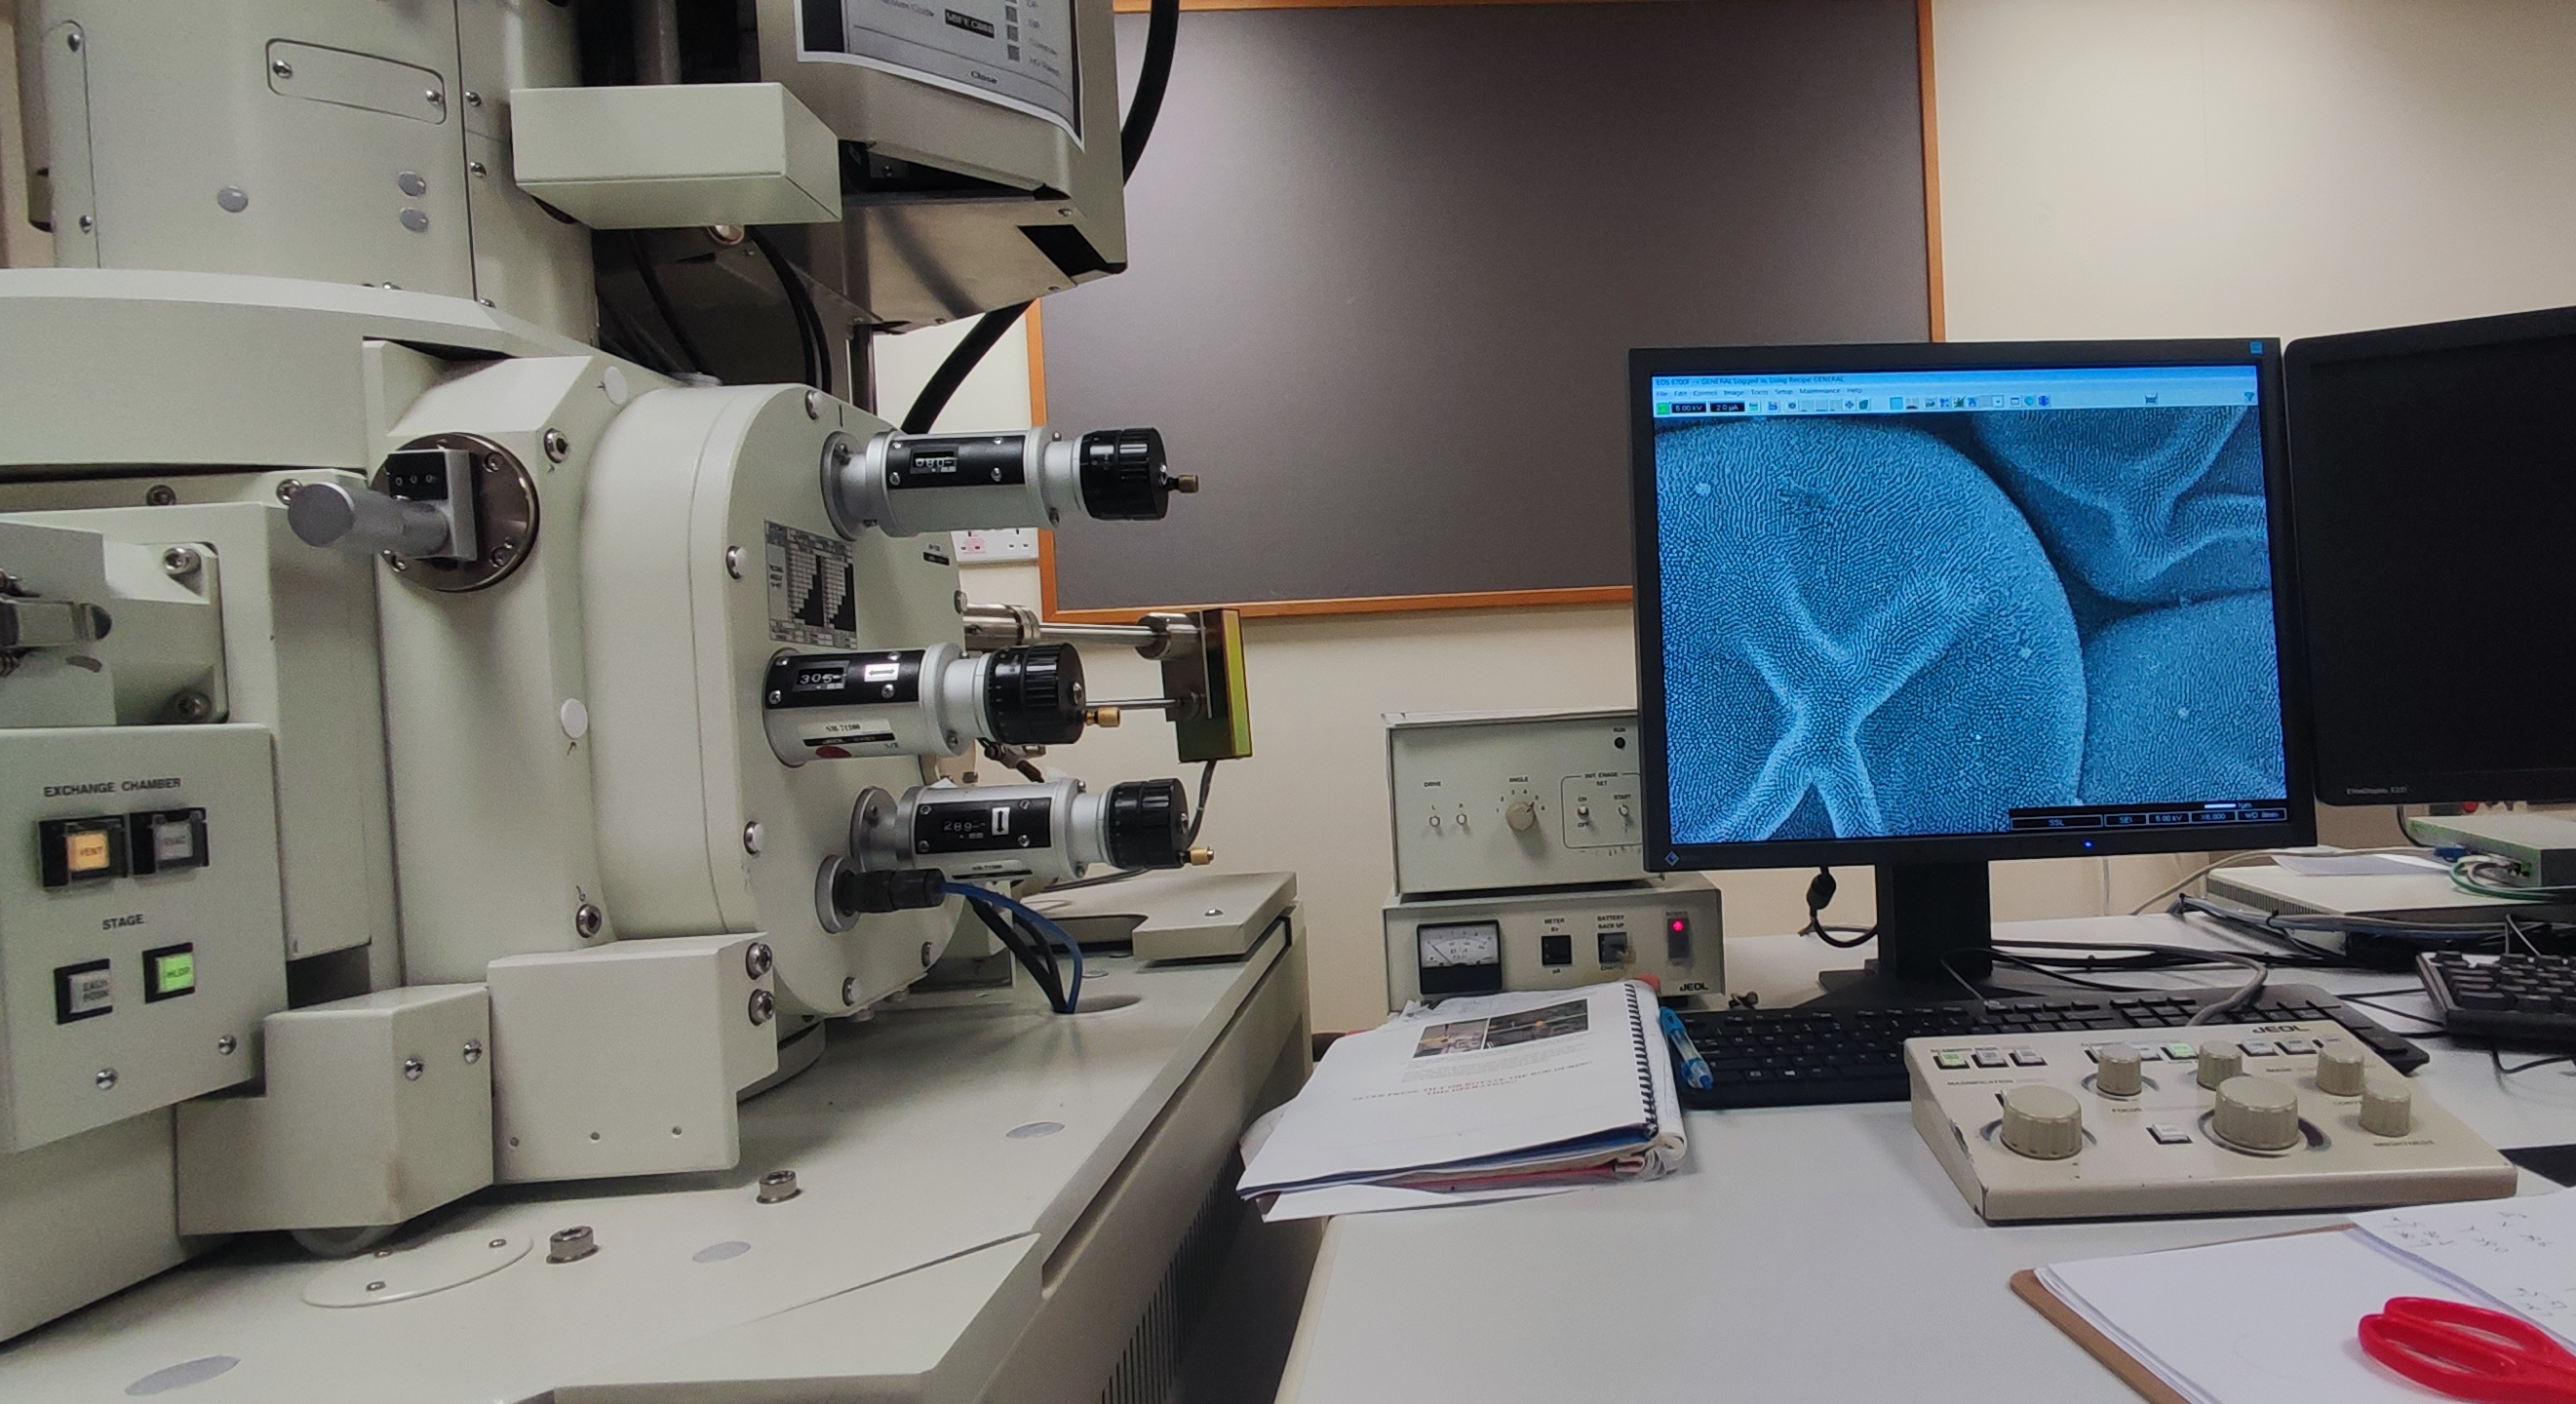
\includegraphics[width=10cm]{images/sem.jpg}
    \caption{Scanning electron microscope}
\end{figure}

Electrons are produced at the top of the column in the electron gun and accelerated through the column at a specified accelerating voltage of 1--30 keV. Condenser lenses and apertures act to reduce the beam diameter. The final lens in the column is the objective lens, which focuses the beam on the sample surface.

The sample itself is mounted on a stage in the chamber area and both the column and the chamber are maintained under vacuum by a combination of pumps. The level of the vacuum will depend on the design of the microscope. Some microscopes allow for variable pumping, allowing the sample chamber to be kept at a lower vacuum level than the rest of the column in order to support low-vacuum imaging.

The position of the electron beam on the sample is controlled by scan coils situated above the objective lens. These coils allow the beam to be scanned over the surface of the sample in the $xy$-plane. The scanned beam strikes the sample, generating a variety of signals including secondary electrons, backscattered electrons, and characteristic X-rays. These signals are then detected by appropriate detectors.

The scan generator, together with an external computer containing specialised software, is able to sync the information from the scan generator (containing the beam’s $x$ and $y$ position at each period in time) with the intensity acquired by the detector, allowing a grayscale image to be displayed and viewed in real time pixel-by-pixel. Depending on the dwell time of the electron beam at each $x$ and $y$ position, the signal-to-noise can be modulated. Magnification results from the size of the scanned area, wherein higher magnifications correspond to progressively smaller scanned areas. The number of pixels may also be adjusted within a given scan area, which can impact the apparent resolution.

\begin{figure}[H]
    \centering
    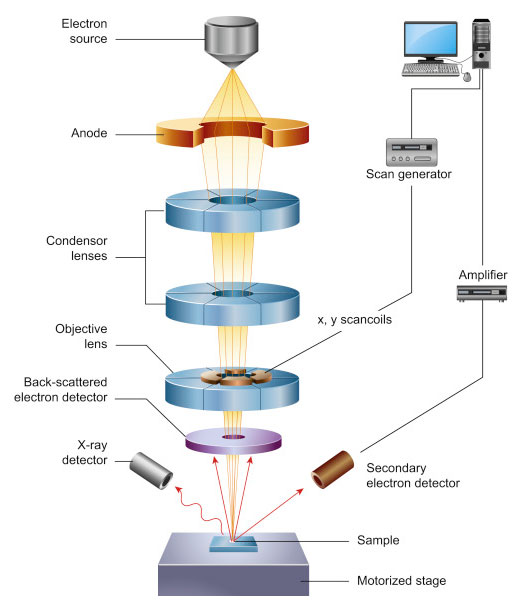
\includegraphics[width=14cm]{images/sem_structure.jpg}
    \caption{Schematic of a scanning electron microscope}
\end{figure}

\begin{figure}[H]
    \centering
    
\includegraphics[width=10cm]{images/sem_mosquito.jpg}
    \caption{Mosquito compound eyes}
\end{figure}

\begin{figure}[H]
    \centering
    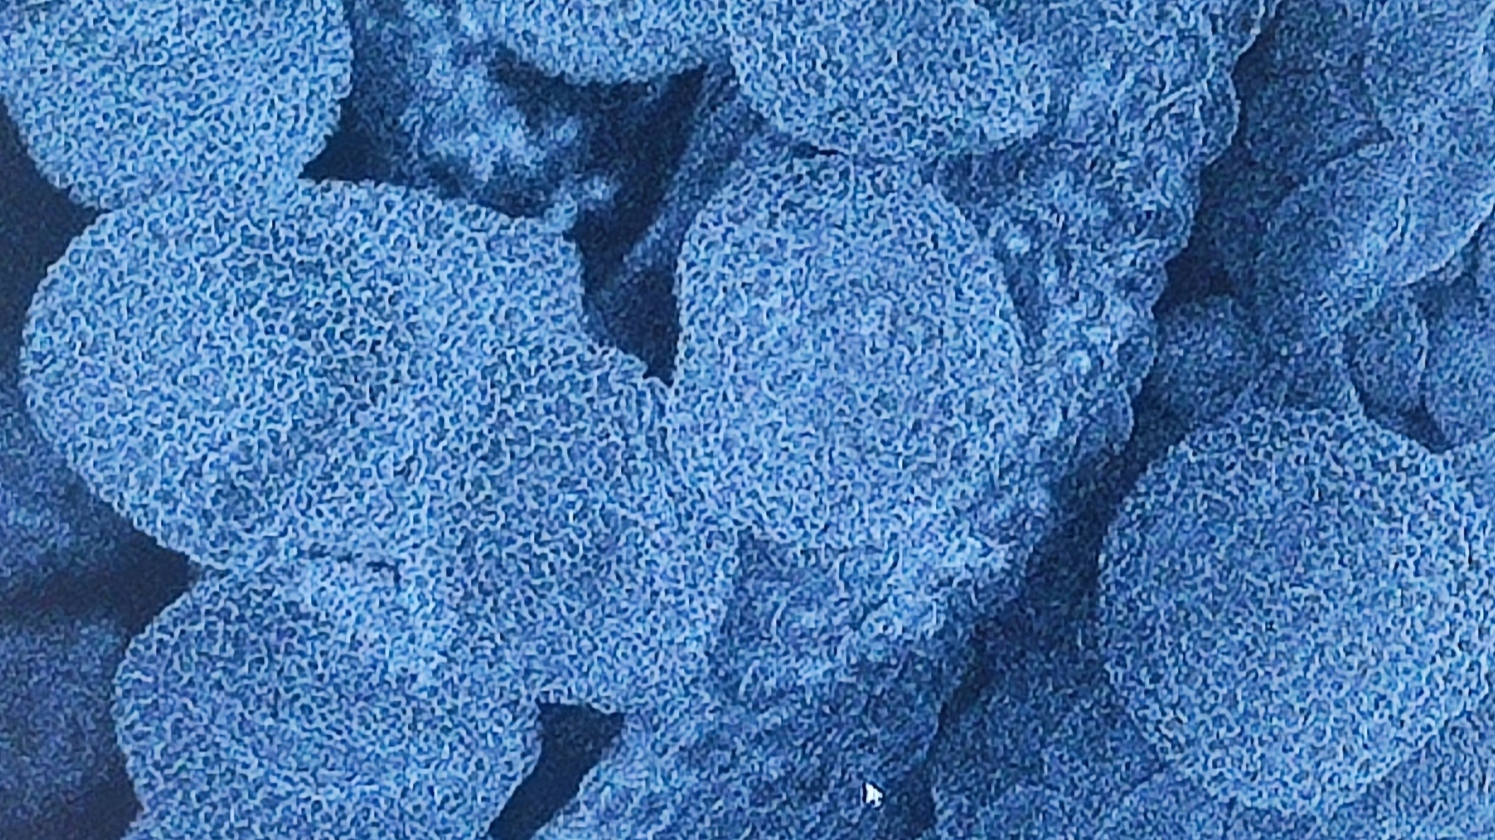
\includegraphics[width=10cm]{images/sem_pollen.jpg}
    \caption{Pollen grains}
\end{figure}
\pagebreak

\section{Research Posters}
Had a look at some research posters in the fields of nanophysics, quantum physics, theoretical physics, and biophysics.

\subsection{Nanophysics}
\subsubsection{The Perfect Imperfection}
Must all atoms be orderly arranged in order to form something useful like a piece of plastic or a football? In the Nanomaterials Research Lab, we don't think so! Can you imagine what happens when we intentionally make something imperfect by switching atoms, displacing, or removing some of these atoms? What will happen to the material? Can we discover new properties that are not observed in the original material? Why yes! We are magicians of the nanoworld, we can intentionally change the compositions of the material when we grow them, or we can focus a laser beam into a tiny spot, just like how a magnifying glass can focus sunlight. The intense heat at the tiny spot is sufficient to break the chemical bond, stirring up the atoms. By moving the laser spot away in a split-second, the matrix undergoes sudden cooling to form a new material with new properties. We have achieved that in 0D, 1D and 2D materials.

\subsubsection{The Nickel-Age of High-Temperature Superconductivity}
Superconductivity is a new phase of matter discovered over a century ago in mercury at just 4 degrees above the absolute zero of temperature. Superconductors have profound applications in high-energy physics and low-energy electronic device technology today due to the zero resistance state leading to zero energy cost to sustain electrical currents. The bottleneck of this application, however, is the extremely low temperature of conventional superconductivity, which is at around -200\degree C colder than the coldest place on Earth. Therefore, research in the ``high-temperature" version of superconductivity has been the holy grail for physicists and engineers. Starting from 1986 the discovery of the ``Copper-age" of high-temperature superconductivity, we recently discovered a new class of materials and open the doorway to the new ``high-temperature Nickel age" of superconductivity.

\subsubsection{Big Questions in Condensed Matter Physics Making Imagination Comes Alive in the Nanoworld}
If you ever doubt your ability to contribute to scientific discoveries due to your age or inexperience, have no doubt. In the Nanomaterials Research Lab, everyone can contribute to new discoveries! It takes some imagination, much hard work, courage to venture into the unknown, determination to search for the answers and passion for what you are striving towards! Don't believe us? Come and take a look at how our junior researchers make their imagination come alive in the Nanoworld!

\subsubsection{2D materials physics: history, development and applications}
Since 2006 the world's first two-dimensional (2D) material (graphene) has been reported, 2D material has been a hot topic in condensed matter physics field for nearly 16 years. At the very beginning, 2D material is commonly considered as an imaginary matter which can't exist in nature. However, with the development of 2D physics, people come to realize a huge potential hidden behind 2D materials. 2D materials consist of several atomic layers in bulk where in each layer atoms are held together by covalent bonds and these layers are interacting via weak van der Waal's interaction. Based on this special structure, 2D materials can be packed together more densely than conventional materials. These materials promise an excellent research platform and they span the entire range of electronic structures from insulators to metal and superconductors. Additionally, 2D materials play important role in transistors, solar cells, and LEDs which run faster and perform better. Currently, 2D physics is still growing fast. Layer dependence of properties of 2D materials is important and it is possible to combine or integrate properties of various 2D materials by constructing heterostructures from individual atomic layers. By stacking 2D materials together and twisting a certain angle, Moir\'{e} superlattice is induced in the crystal structure which leads to another revolution in 2D materials field. Various 2D materials are reported these years and each has unique physical and chemical properties, providing rich resources for further research.
\pagebreak

\subsection{Quantum Physics}
\subsubsection{Seismic Sensing with Optical Fibres}
Michelson interferometers utilise the interference of light beams between its two arms to determine their length difference with a sub-wavelength precision. It is possible to use optical fibres to guide light in the two arms, and to subsequently measure the relative length changes of the optical fibres. However, Michelson interferometers are unable to distinguish the direction of length changes between both arms. This can be resolved by modulating the interference signal of the carrier signal, where the direction and magnitude of length change is then encoded into the phase of the carrier signal. This is done by modulating the frequency of the light on one arm of the interferometer, and the absolute length difference between both arms is thus encoded into the phase of the interference signal. We call such a setup a heterodyned fibre- based phasemeter. This measurement strategy is known as a heterodyne detection. A deployed optical fibre in the ground experiences strain from environmental sources, which we can then detect hrough such a phasemeter. With our setup, we try to find out to what extent existing optical fibers can be used to detect seismic events like earthquakes.

\subsubsection{From Qubits to Cats: Unravelling the physics of cQED}
This poster introduces high school students to the fascinating world of Circuit Quantum Electrodynamics (QED), focusing on the fundamental physics of its building blocks such as the qubit transmon, resonators, and their interconnections. Delving into the realm of quantum mechanics, it explores the creation of 'cat states', a captivating concept where quantum systems exist in superposition, akin to Schr\"{o}dinger's famous thought experiment involving a cat in two states simultaneously. By presenting simplified explanations and illustrative diagrams, this poster aims to spark curiosity and lay the groundwork for understanding the intriguing concepts within quantum physics, paving the way for a deeper exploration of cutting-edge technologies in the field of quantum computing and quantum information science.

\subsubsection{Quantum Ingenuity Unleashed: Gears of Quantum Computing}
This poster aims to introduce JC students to the experimental hardware used in circuit quantum electrodynamics (cQED) research. The poster will include sections on superconductivity, Josephson junctions, flux-tunable qubits, temperature effects, and the design of a device and chip for experiments at mK temperatures (using dilution refrigerator). The goal is to provide students with a basic understanding of the advanced technology and techniques used in cutting-edge quantum research, and to inspire them to pursue further studies and careers in this exciting field.
\pagebreak

\subsection{Theoretical Physics}
\subsubsection{The Quantum Physics of Black Holes and Emergence of Space and Time}
Arguably the biggest question in fundamental physics today is how does spacetime, that is, the fabric of reality, emerge from nothing. One of its leading proposals, as suggested by string theory, is that ER = EPR, or rather, wormholes = quantum entanglement. In other words, spacetime emerges from quantum entanglement, whence information is even more fundamental than spacetime itself.
\pagebreak

\subsection{Biophysics}
\subsubsection{A Guide to Magnetic Tweezers and Their Applications on DNA manipulations}
Nowadays, magnetic tweezers are widely used to investigate various protein-nucleic acid systems. These studies encompass a wide range of subjects, including helicases, DNA polymerases, topoisomerases, gyrases, cellular and viral RNA polymerases, nucleoprotein filaments, and the mechanical stability of protein folding and protein-ligand interactions. The technique's simplicity and robustness contribute to its popularity as a powerful single-molecule force spectroscopy assay within the academic community.
\pagebreak

\section{Career Prospects}
{\color{red}\textit{Lecturer}}: \href{https://www.physics.nus.edu.sg/faculty/wang-qinghai/}{Dr. Wang Qinghai}

The National University of Singapore (NUS) admits about 50 students annually into its Physics programme, a course under the Faculty of Science (FoS).

At the university level, education often falls into two distinct categories:
\begin{itemize}
\item Professional education

This type of education is tailored to prepare students for specific professions or careers. It offers specialised training, skill development, and knowledge aligned with particular industries or vocations. 

Examples: medicine, law, engineering, accounting.

\item General education

General education provides a broader and more diverse academic experience. It doesn't aim at training individuals for a particular job or profession but instead focuses on imparting foundational knowledge, critical thinking skills, and a broad understanding of various disciplines. It is about fostering a well-rounded education that encourages exploration, interdisciplinary connections, and adaptability in different fields.

Examples: physics, mathematics
\end{itemize}

The \textbf{graduate employment survey} consists of data for various courses regarding the percentage of graduates who have a full-time permanent (FTP) job, go for further studies, and median income. \cref{table:survey} shows the data for the year 2022.
\begin{table}[H]
\centering
\begin{tabular}{cccc}
\hline\hline
& FTP job & Further studies & Median income \\
\hline
FoS & 71\% & 12\% & -- \\
Physics & 58\% & 29\% & \$4509 \\
DSA & 91\% & 6\% & \$5500 \\
\hline\hline
\end{tabular}
\caption{Graduate employment survey 2022}
\label{table:survey}
\end{table}

No specific FTP job for Physics graduates. Job prospects span diverse sectors such as corporate roles, research positions, teaching, and opportunities in entrepreneurial ventures.

Top employers for FTP employed Physics graduates ($N=22$)
\begin{itemize}
\item Accenture PLC
\item Bank Julies Baer \& Co. Ltd.
\item Global Foundries Inc.
\item Institute of High Performance Computing
\item Mediatek Singapore Pte. Ltd.
\item Micron Technology, Inc.
\item Ministry of Education
\item National University of Singapore
\item NCS Pte. Ltd.
\item Research Management -- National University of Singapore
\item Rystad Energy
\item Squarepoint Capital LLP
\item Systems on Silicon Manufacturing Company Pte. Ltd.
\item Visa Inc.
\item World Scientific Publishing
\end{itemize}

Top roles for FTP employed Physics graduates ($N=22$)
\begin{itemize}
\item Research Officer (non-statistical)
\item Manufacturing Engineer (general)
\item Quality Control / Assurance Engineer
\item Assistant Engineer
\item Editor (news and periodicals)
\item Electronics Engineer
\item Financial Analyst (e.g. equities analyst, credit analyst, investment research analyst)
\item General Office Clerks
\item Information Technology Testing / Quality Assurance Specialist
\item Management Consultant
\item Primary School teacher
\item Private Tutor (Academic)
\item Production Engineer
\item Research and Development Manager
\item Secondary School Teacher (including Integrated Programme Year 1 -- 4 Teacher)
\item Software Developer / Engineer (including Blockchain and Cryptography Developer / Engineer / Architect)
\item Systems Designer / Analyst
\item Technical / Vocational / Commercial Education Institute Teacher and Trainer
\end{itemize}


\pagebreak

\section{Alumni Panel}
Three alumni of NUS Physics were invited for a sharing.

\begin{enumerate}
\item Dr. Da Yang Tan

Lecturer with NUS College, National University of Singapore

(B.Sc.) Physics National University of Singapore (2012) \\
(Ph.D.) Physics National University of Singapore (2016)

Da Yang is a Ph.D. graduate from NUS Physics, specialising in open quantum systems. He pioneered work in enabling large-scale unmanned aircraft operations at NTU's Air Traffic Management Research Institute. Transitioning to education, he revamped post-graduate diploma courses in Mathematics at NIE. Currently, Da Yang is a lecturer at NUS College, specialising in science and mathematics education. His research focuses on complex systems in education.

\item Dr. Tan Hong Qi

Senior Medical Physicist, National Cancer Centre Singapore

(B.Sc.) Physics National University of Singapore (2013) \\
(Ph.D.) Physics National University of Singapore (2018)

Tan Hong Qi joined NCCS in 2018 and is currently a senior medical physicist in the department of radiation oncology. He has received several awards and recognitions, including the IAEA fellowship in 2022, SingHealth AHP young discoverer award in 2021, SEAFOMP Young Leader award in 2023, and the IUPAP early career scientist award in 2023. He is also a diplomate of IMPCB and a clinical instructor at Duke--NUS. He has represented Singapore as an expert in the IAEA technical meeting on radiation protection and led the medical physics research group in NCCS.

\item Mr. Timothy Lim Chun Gao

Engineer at Hometeam Science

(B.Sc.) Physics National University of Singapore (2023)

Timothy got the physics prowess to back up Home Team Departments in the high-tech realm of Biometrics Technology. To ensure that Singapore stays ahead in this increasingly complex landscape, innovative technology is crucial to empower the Home Team to operate effectively and impact exponentially.
\end{enumerate}
\end{document}
